\begin{lstlisting}[escapechar=|,language=C]
for (j = 0; j < |{\bf m}|; j++) {
  d = 0.0;
  for (k = |{\bf rowstr }|[j]; k < |{\bf rowstr}|[j+1]; k++)
    d = d + |{\bf a}|[k]*|{\bf z}|[|{\bf colidx}|[k]];
  |{\bf r}|[j] = d; }
\end{lstlisting}
\vspace{-1em}
\begin{lstlisting}[escapechar=|,language={LLVM},basicstyle=\linespread{0.939}\tiny\ttfamily]
; <label>:2:
  %j = phi i64 [ %j_next, %12 ], [ 0, %1 ]
  %j_cond = icmp slt i64 %j, |{\bf \%m}|
  br i1 %j_cond, label %3, label %13|\vspace{1mm}|
; <label>:3:
%4 = getelementptr i32, i32* |{\bf \%rowstr}|, i64 %j
  %5 = load i32, i32* %4
  %j_next = add nuw nsw i64 %j, 1
  %6 = getelementptr i32, i32* |{\bf \%rowstr}|, i64 %j_next
  %7 = load i32, i32* %6
  %k_begin = sext i32 %5 to i64
  %k_end = sext i32 %7 to i64
  br label %8|\vspace{1mm}|
; <label>:8:
  %k = phi i64 [ %k_next, %9 ], [ %k_begin, %dnext ]
  %d = phi double [ 0.0, %3 ], [ %d_next, %9 ]
  %k_cond = icmp slt i64 %iv, %k_end
  br i1 %k_cond, label %9, label %12|\vspace{1mm}|
; <label>:9:
  %a_addr = getelementptr double, double* |{\bf \%a}|, i64 %k
  %a_load = load double, double* %a_addr
  %cix_addr = getelementptr i32, i32* |{\bf \%colidx}|, i64 %k
  %cix_load = load i32, i32* %cix_addr
  %10 = sext i32 %cix_load to i64
  %z_addr = getelementptr double, double* |{\bf \%z}|, i64 %10
  %z_load = load double, double* %z_addr
  %11 = fmul double %a_load, %z_load
  %d_next = fadd double %d, %11
  %k_next = add nsw i64 %k, 1
  br label %8|\vspace{1mm}|
; <label>:12:
  %r_addr = getelementptr double, double* |{\bf \%r}|, i64 %j
  store double %d, double* %r_addr
  br label %2
\end{lstlisting}
\vspace{-0.287cm}
\caption{Sparse linear algebra in C and LLVM IR}
\label{fig:spmvexample1}
%\end{figure}

\centering
\vspace{0.0em}
{\centering
\begin{minipage}{0.05\linewidth}
\vspace{0pt}
\centering
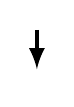
\begin{tikzpicture}[ultra thick]
 \draw [black,   -latex      ] (0,0.5) -- (0,0) node [] {};
\end{tikzpicture}
\end{minipage}
\begin{minipage}{\linewidth}
% \vspace{-5pt}
\centering
\textbf{Idiom detection with IDL program in \Cref{fig:spmv}}
\end{minipage}
\begin{minipage}{0.05\linewidth}
\vspace{0pt}
\centering
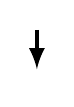
\begin{tikzpicture}[ultra thick]
 \draw [black,   -latex      ] (0,0.5) -- (0,0) node [] {};
\end{tikzpicture}
\end{minipage}
}

%\begin{figure}
{\centering
\footnotesize 
\begin{tabular}{l|l}
\textbf{Variable Name} & \textbf{Assigned IR Value}\\
\hline
iterator                    & \texttt{\%j}\\
inner.iter\_begin           & \texttt{\%k\_begin}\\
inner.iter\_end             & \texttt{\%k\_end}\\
inner.iterator              & \texttt{\%k}\\
idx\_read.value             & \texttt{\%cix\_load}\\
indir\_read.value           & \texttt{\%a\_load}\\
seq\_read.value             & \texttt{\%z}\\
\end{tabular}
\hspace{0.5cm}
\begin{tabular}{l|l}
\textbf{Variable Name} & \textbf{Assigned IR Value}\\
\hline
output.address              & \texttt{\%r\_addr}\\
iter\_begin                 & \texttt{0}\\
iter\_end                   & \texttt{\%\bf m}\\
idx\_read.base\_pointer     & \texttt{\%\bf colidx}\\
seq\_read.base\_pointer     & \texttt{\%\bf a}\\
indir\_read.base\_pointer   & \texttt{\%\bf z}\\
\dots                       & \dots\vspace{-0.5mm}\\
\end{tabular}

}

\caption{Constraint solution for sparse mv}
\label{fig:spmvexample2}
%\end{figure}

\centering
\vspace{0.0em}
{\centering
\begin{minipage}{0.05\linewidth}
\vspace{0pt}
\centering
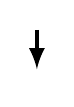
\begin{tikzpicture}[ultra thick]
 \draw [black,   -latex      ] (0,0.5) -- (0,0) node [] {};
\end{tikzpicture}
\end{minipage}
\begin{minipage}{\linewidth}
% \vspace{-5pt}
\centering
\textbf{Code generation: insert arguments, replace code}
\end{minipage}
\begin{minipage}{0.05\linewidth}
\vspace{0pt}
\centering
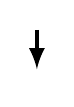
\begin{tikzpicture}[ultra thick]
 \draw [black,   -latex      ] (0,0.5) -- (0,0) node [] {};
\end{tikzpicture}
\end{minipage}
}


%\begin{figure}
\begin{lstlisting}[escapechar=|,mathescape,commentstyle=\color{gray}\itshape,language=C]
cusparseDcsrmv(context,
    CUSPARSE_OPERATION_NON_TRANSPOSE, |{\bf m}|, n,
    |{\bf rowstr}|[|{\bf m}|+1]-|{\bf rowstr}|[0], &gpu_1, descr, gpu_|{\bf a}|,
    gpu_|{\bf rowstr}|, gpu_|{\bf colidx}|, gpu_|{\bf z}|, &gpu_0, gpu_|{\bf r}|);
\end{lstlisting}
\vspace{-0.287cm}
\caption{Generated function call to cuSPARSE}
\label{fig:spmvexample3}